\chapter{Introduction}

We show how the process by which people drive markets to a sustained and stable equilibrium of
aggregate supply and aggregate demand is constrained and destabilized by technical properties of the
currency used. We identify the major technical problems with legacy currencies and present a design
for an significantly improved currency that is highly likely to maintain a sustained and stable
state with aggregate supply in equality with aggregate demand and full-employment.

Around 1777 David Hume observed, despite theoretical considerations to the contrary, that properties of
a nation's currency had observable affects on the state of the economy,

\begin{quotation}
If we consider any one kingdom by itself, it is evident, that the greater or less plenty of money is
    of no consequence; since the prices of commodities are always proportioned to the plenty of
    money, and a crown in Harry VII.’s time served the same purpose as a pound does at present ...
    It is indeed evident, that money is nothing but the representation of labour and commodities,
    and serves only as a method of rating or estimating them. Where coin is in greater plenty; as a
    greater quantity of it is required to represent the same quantity of goods; it can have no
    effect, either good or bad, taking a nation within itself; any more than it would make an
    alteration on a merchant’s books, if, instead of the Arabian method of notation, which requires
    few characters, he should make use of the Roman, which requires a great many ... \textbf{But notwithstanding this conclusion}, which must be allowed just, it is certain, that, since the
    discovery of the mines in America, industry has encreased in all the nations of Europe, except
    in the possessors of those mines; and this may justly be ascribed, amongst other reasons, to the
    encrease of gold and silver.  Accordingly we find, that, in every kingdom, into which money
    begins to flow in greater abundance than formerly, every thing takes a new face: labour and
    industry gain life; the merchant becomes more enterprising, the manufacturer more diligent and
    skilful, and even the farmer follows his plough with greater alacrity and attention. This is not
    easily to be accounted for, if we consider only the influence which a greater abundance of coin
    has in the kingdom itself, by heightening the price of commodities, and obliging every one to
    pay a greater number of these little yellow or white pieces for every thing he purchases.
\end{quotation}

Hume's considerations suggest that any effective economic model requires an understanding of both
how people interact with others, changing their individual economic agreements in a way that pushes
markets toward equilibrium of supply and demand, but also an understanding of the role of money as
an essential tool is those market transactions.

Considering the economic process in the absence of currency, the process of supply and demand as we
understand it, infers a macro-economic equilibrium where aggregate demand and aggregate supply are
in equllity, i.e. that if we aggregate excess supply and demand across markets, they should average
out to close to zero.

[more details here]




However, contrary to Figure \ref{fig:supply_and_demand_prediction} which implies full-employment
Figure \ref{fig:ui_all_data} shows a vastly differing results.

\begin{figure}[H]
\centering

\includegraphics[scale=0.48]{blank}
\caption{Inflation Rate vs. Unemployment Data}
\label{fig:ui_all_data}
\end{figure}

[asymmetry diagram].

Positive rates of unemployment are so consistent across all countries and throughout the decades of
recorded economic history, to such an extent that unemployment appears as solid as physical law.

Economic theorists have been seeking a solution to this problem for many years without success.
Considering that any currency mechanism is absent from this model of supply and demand, despite
Hume's obversations suggest currencies have significant effects, it seems reasonable to find a way
to include currency in our model. This leads to the question of what methods should be used to
analyze the properties of currency. The fundamental insight that we present is that because currency
is a digital system, the way to approach its analysis is roughly analogous to the way we approach
the analysis and design of other digital systems (the internet being an interesting example), i.e.
that we should approach the analysis of currency as an engineering problem, and in particular the
engineering and control of dynamic systems. 

Economic theory approaches economic problems similarly to the way medicine treats the human body, by
applying relatively small changes, such as medicine, in response to various pathologies.
Destructuring and rebuilding biological systems is impossible. Importantly however, the control
system for economies, the currency, can indeed be destructured and rebuilt from first principles.
Thus we take a different approach, viewing currency more like a robotics problem, something that can
be built from the bottom up.

\subsection{Transactions}

Even if we have considerable control over the currency mechanism, such as requiring transactions to
conserve purchasing power,  we are limited in our ability to control the \textbf{use} to which a
currency is put. Historical experience is a good guide to the main uses which people use money for,
and these can be categorized into various types of transactions. The simplest and most fundamental
transaction are exchange transactions as shown in figure \ref{fig:exchange_transaction1}.

\begin{figure}[H]
\centering
\includegraphics[scale=0.60]{01_introduction/png/exchange_transaction}
\caption{Exchange Transaction}
\label{fig:exchange_transaction1}
\end{figure}

We can consider exchange transactions as occuring at a point in time, where goods or services are
exchanged for currency. Another common type of transaction we will call a time transaction,

\begin{figure}[H]
\centering
\includegraphics[scale=0.60]{01_introduction/png/time_transaction}
\caption{Time Transaction}
\label{fig:time_transaction1}
\end{figure}

where at time $t_0$ money is borrowed and used to make an exchange transaction of currency in
exchange for goods and service. At a later time $t_1$, the principal and interest is repaid to the
lender. The third transaction category we call contract transactions. Contract transactions are
characterized by a transfer of money in return for a change in owner of contractural obligations.

\begin{figure}[H]
\centering
\includegraphics[scale=0.60]{01_introduction/png/contract_transaction}
\caption{Contract Transactions}
\label{fig:contract_transaction1}
\end{figure}

Contractural transactions and variations on them can become complex. Transactions are not limited to
these categories. We will examine some other transaction categories later in the paper.

\subsection{Feedback Regulators}

\begin{figure}[H]
\centering
\includegraphics[scale=0.60]{01_introduction/png/feedback_schema}
\caption{Economic Feedback Schema}
\label{fig:feedback_schema1}
\end{figure}

A general control system schema with a single control variable can be represented as

\begin{figure}[H]
\centering
\includegraphics[scale=0.60]{01_introduction/png/economic_feedback_schema}
\caption{Economic Feedback Schema}
\label{fig:economic_feedback_schema1}
\end{figure}

A set of possible transactions provides an interface to the currency's accounts. In designing a
digital currency, we have considerably more control over the way in which accounts are used,
compared to a paper currency where everyone is free to exchange units of currency. The currency also
consists of a 
also a feedback mechanism, controlled algorithmically or through a monetary authority, to regulate
aggregate demand. The process by which people drive markets to an equilibrium of aggregate supply
and aggregate demand occurs in the Market Activity box. This process which we think of as the
central driver of market activity, is internal to currency feedback mechanism. As we will show, the
design of the currency constrains can prevent this process from reaching equilibrium and we
required further regulatory mechanisms built into the currency.

\subsection{Results}

% Move this to "Exchange_Transactions_and_Errors".
%
% As required in the analysis of all engineering systems, we look at the effects of the second law of
% thermodynamics on our system in the form of errors or noise. We find that that an error rate that
% reduces aggregate agreements can only be compensated for by increases in aggregate demand. This is
% somewhat analogous to airlines overbooking in order to compensate for cancellations. Overbooking
% will only occur if airlines set prices so that the demand for seats is greater than the supply of
% seats. At the aggregate level an excess aggregate demand can only be driven by constantly increasing
% aggregate demand at a certain rate. Claude Shannon's information theory determines the extent to
% which an error rate can be reduced by adding redundancy (in our case excess aggregate demand) to the
% system.


% How much detail to we put here? I have decided only to put the requirements, because at get an
% intuitive understanding of what is happening we need to work through 02 dynamic systems,

Engineering methods are applied to the the currency mechanism not the behaviour of people. The only
assumptions made about people's decision-making processes and the basic tenets of supply and demand
interaction, that people drive markets to equilibrium (and this assumption itself is confirmed when
we test the theory against data (\ref{section:data})). In the remainder of the paper by start with
the the currency control system as shown in Figure \ref{fig:economic_feedback_schema1}, and
step-by-step take each transaction category, introduce it into the model and apply engineering
analytical methods. As a result of this process we find the following requirements, 

1. Aggregate demand must be continuously increasing at a rate sufficient to compensate for errors.
Without this requirement the currency constrains the transaction possibility space of markets,
preventing people from driving markets to macro-economic equilibrium.

2. All units written into contracts must be independent of the price level. Without this condition a
positive feedback instability can result in runaway behaviour under increases in the inflation rate.

3. Contract transactions must be prevented. Without this condition contract transactions can result
in runaway behaviour in prices, difficulties in controlling an overly complex system. Preventing
contract transactions allows for a currency design with precise control over aggregate demand.

\subsection{Implementation}
    
There appear to be effective design solutions to meet these requirements.

In the absence of contract transactions a unique global value, a \emph{Demand Index} $D_x$ can be
used by a central monetary authority or by algorithm to precisely control aggregate demand. Accounts
store a base value and payments are in purchase value, demoninated in a unit (such as \verb|$|) that
is a product of the base value and the demand index. In general the base value is hidden from users
and accounts appear as purchasing value.

The \emph{Price Index} $P_x$ is regularly published, and all legal contracts must be written in a
unit of account of constant purchasing power. This setup has been used in Chile for several decades
for almost all contracts and has proven practical even when being used with a paper currency. With
thus unit of account in place, the aggregate demand of a currency can be directly controlled and
variable rates of inflation without risk of runaway behaviour. 

A digital currency can be designed to distinguish between exchange transactions and time
transactions.

Exchange transactions would require both the buyer and lender to record the quantity of goods and
services purchase. This record could also be used by sellers and buyers to record agreements, but
the use of cryptographic methods to prevent such purchase data being available to others except
those directly involved in the transaction is required. This mechanism would also ensure that
accurate price and quantity data could be recorded for the calculation of a Price Index. 

Time transactions would require the same conditions as an exchange transaction, but also that the
repayment schedule is determined at the time of the initial loan payment, and that the recipient of
the loan repayment is the same account from which the load payment was made.

This would generally prevent the use of contract transactions which require that the recipient of
repayment changes. It is still possible for people to make informal contracts, and to obfuscate the
initial loan payment and repayments as exchange transactions, by recording a false good or service.
This however, would forgo both parties any right to legal process in the case of a dispute, because
the transactions are clearly marked as an exchange, with no further contractural obligations.


% Given this set of 'primitives' we no reconstruct  our control system, introducing each component
% one at a time and carefully analyzing their interaction with each other.










% % Figure _ shows a schema where we introduce the most common transactions. 
% 
% % The box represents the process by which people adjust price and quantity to reach a set of
% % transactions. We take the simplest model and supply and demand which implies that people react to
% % excess aggregate supply or excess aggregate demand and adjust prices and quantities of
% % transactions is such a way on average aggregate supply and aggregate demand are in equality.    
% 
% % Given this, we then step-by-step introduce different categories of transactions into our model,
% % the first being exchange transactions.
% 
% % We also introduce the basic mathematics of exchange transactions that relates individual exchange
% % transactions to aggregate properties.
% 
% \begin{figure}[H]
% \centering
% \includegraphics[scale=0.28]{/01/exchange_only_feedback_schema}
% \caption{Exchange Only Feedback Model}
% \label{fig:exchange_only_feedback_schema1}
% \end{figure}
% 
% In \autoref{chapter:exchange_transactions_and_errors} we consider the effects of errors on this
% system. All digital systems in some way rely on methods to correct for errors. Claude Shannon's
% information theory shows the mathematical limits on the minimum redundant information required to
% compensate for loss of information due to errors in a communication channel. We examine the effects
% of an error rate that reduces the set of agreed transactions in a given time period to actual
% transactions. We show that excess proportional aggregate supply equal to the unemployment rate
% depends on maining redundancy though an excess proportional aggregate demand. In the situation where
% the growth rate is zero, this excess proportional aggregate demand maps directly to the inflation
% rate. Increases in the growth rate result in lower inflation rates to compensate for errors.
% Decreases in the growth rate result in higher inflation rates required to compensate for errors.
% Figure TODO indicates the technical constraints that an error rate limits the space over which the
% dynamic process of supply and demand human economic interactions can play out.
% 
% \begin{figure}[H]
% \centering
% 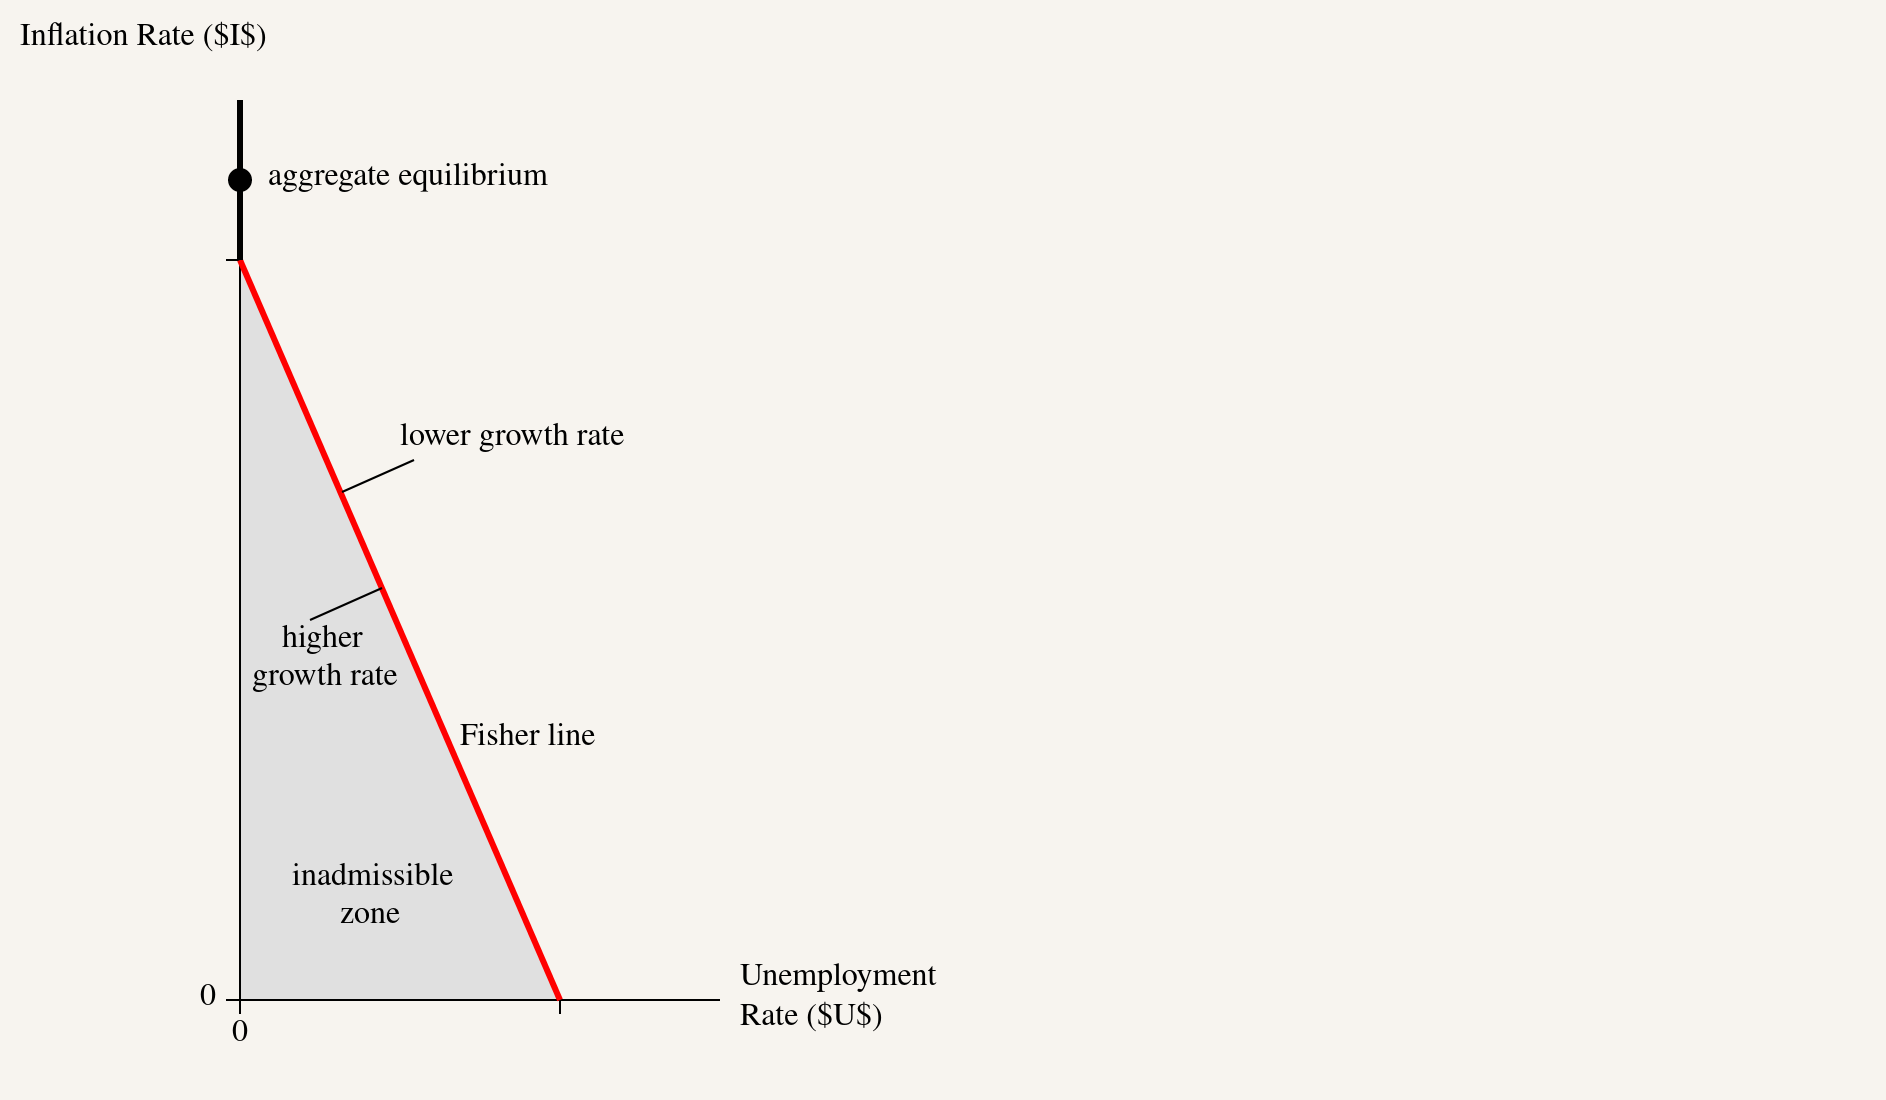
\includegraphics[scale=0.28]{/01/error_model}
% \caption{Error Model}
% \label{fig:error_model1}
% \end{figure}
% 
% 
% Detailed unemployment rate and inflation rate data is available for many countries over long periods
% of time, and so in \autoref{chapter:data} we will hold up this hypothesis against measurement.
% Before that we will introduce an new category of transactions, time transactions, to our model. For
% each new category of transactions we add to our model we need to consider the way that these new
% transactions interact with all other categories of transactions.
% 
% In \autoref{chapter:time_transactions}
% 
% In \autoref{chapter:data}
% 
% In \autoref{chapter:external_transactions}
% 
% In \autoref{chapter:contract_transactions} we look at transactions where contracts are exchanged for
% money. A positive feedback instability can occur when the price of contracts of some kind is rising
% over time, inducing further increase in the prices/interest rates on these contracts. These
% instabilities have effects on time transactions but more critically, destabilize a currency's
% requirement to effectively control aggregate demand so as to maintain aggregate equilibrium. The
% aggregate behavior of contract transactions is fundamentally unpredictable due to positive feedback
% instabilities and the unlimited complexity of contractural arrangements. Under conditions where
% contract transactions are severely limited, but still allowing time transactions, we introduce a
% method to precisely control aggregate demand.
% 
% In \autoref{chapter:other_transactions}
% 
% In \autoref{chapter:implementation}
% 
% \subsection{Destructuring and Negative Feedback}
% 
% \begin{figure}[H]
% \includegraphics[scale=0.28]{/01/feedback_schema}
% \caption{Control System Schema with Actuator}
% \label{fig:feedback_schema}
% \end{figure}
% 
% In systems that don't require an additional source of energy to control the system, the actuator can
% be removed from the feedback schema,
% 
% \begin{figure}[H]
% 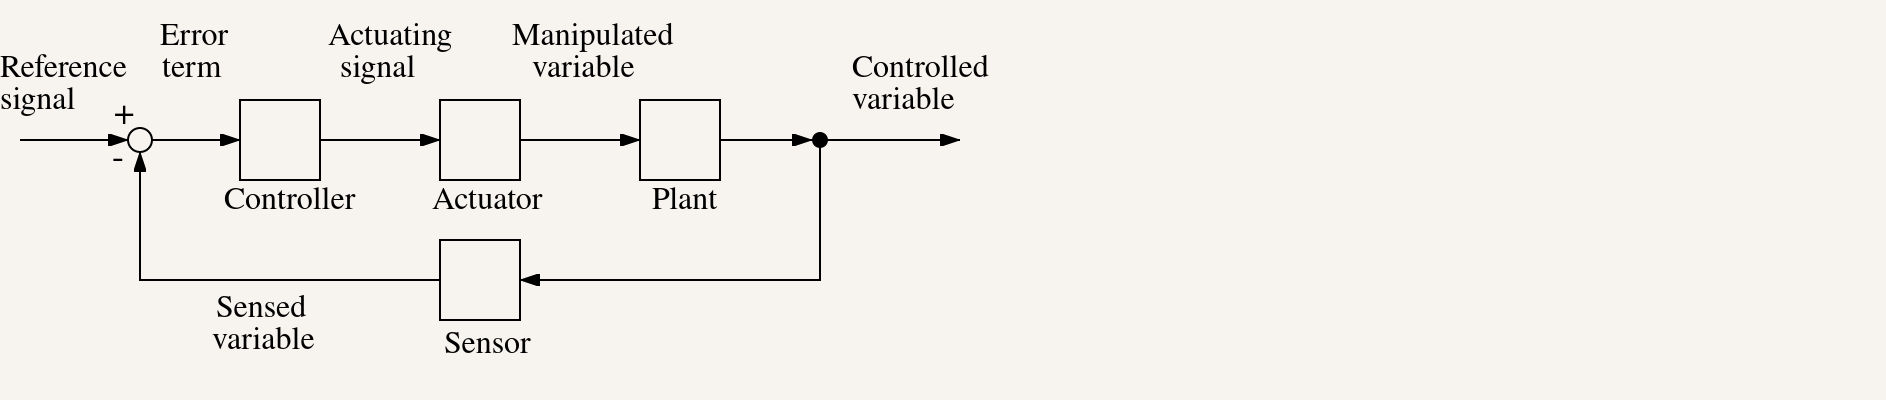
\includegraphics[scale=0.28]{/01/feedback_schema_no_actuator}
% \caption{Control System Schema}
% \label{fig:feedback_schema_no_actuator}
% \end{figure}
% 
% A simple example of a control system is a thermostat which adjusts the heating of a room. Some
% condition of the plant (the thing we want to control) is controlled by measuring the state of the
% plant and feeding back into the plant the difference between this state and the desired state (the
% reference signal). The design of control systems have the general guiding properties that dictate
% our design approach, namely that our ability to correctly model the plant, stems must be able to
% correct for errors, noise and/or energy disipation in the plant and the the minimum number of
% control variables is determined by the number of variables that the control system seeks to control.
% A control system for the economy looks like Figure \ref{fig:economic_feedback_schema}.
% 
% \begin{figure}[H]
% \centering
% \includegraphics[scale=0.28]{/01/economic_feedback_schema}
% \caption{Control System Schema for an Economy}
% \label{fig:economic_feedback_schema}
% \end{figure}
% 
% Zooming into the currency box in Figure \ref{fig:economic_feedback_schema}, we can specify the
% classes of transactions that a currency implements. Transaction classes include the exchange of
% money in return for goods or services, lending money now in exchange for payment later, and
% exchanging money in exchange for a change in a contract. This way of viewing currency indicates a
% control problem because the system has a single means to control money supply, but at least four
% classes of components that require control and interact with the other classes.
% 
% \subsubsection{Control Problem}
% 
% \begin{figure}[H]
% \centering
% 
\includegraphics[scale=0.48]{01_introduction/png/blank}
% \caption{Control Problem}
% \label{fig:control_problem}
% \end{figure}
% 
% The passing around of paper currency, in conjunction with contract agreements, is used to carry
% out many kinds of transactions, the four main classes we term exchange transactions, time
% transactions, contract transactions and external transacation. Each class of transaction interacts
% with the other classes in complex ways. The fundamental problem is that these interactions are
% overly complex to control with a single control such as control of the money supply. In general,
% control systems require one control variable for each property of the plant that requires control.
% This is implicit in the name of control systems, SISO for single input single output, MIMO for
% multiple input multiple output. We therefore take a systematic approach to this control problem,
% destructuring each transaction class and examining the way it interacts with other transactions
% classes, step by step.
% 
% \begin{figure}[H]
% \centering
% 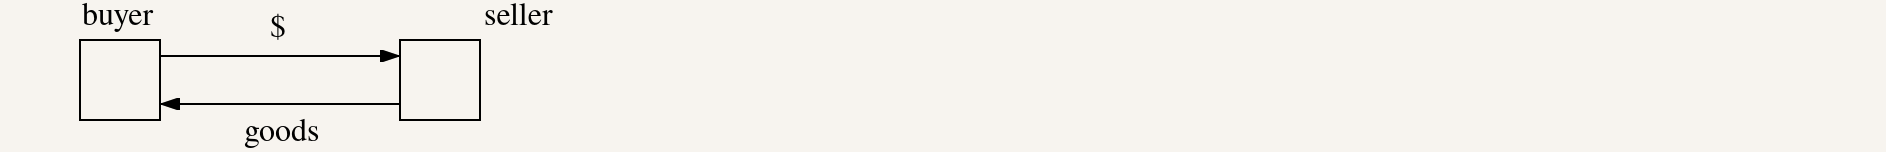
\includegraphics[scale=0.28]{01_introduction/png/exchange_transactions}
% \caption{Exchange Transactions}
% \label{fig:exchange_transactions}
% \end{figure}
% 
% \begin{figure}[H]
% \centering
% 
\includegraphics[scale=0.48]{blank}
% \caption{Time Transactions}
% \label{fig:time_transactions}
% \end{figure}
% 
% \begin{figure}[H]
% \centering
% 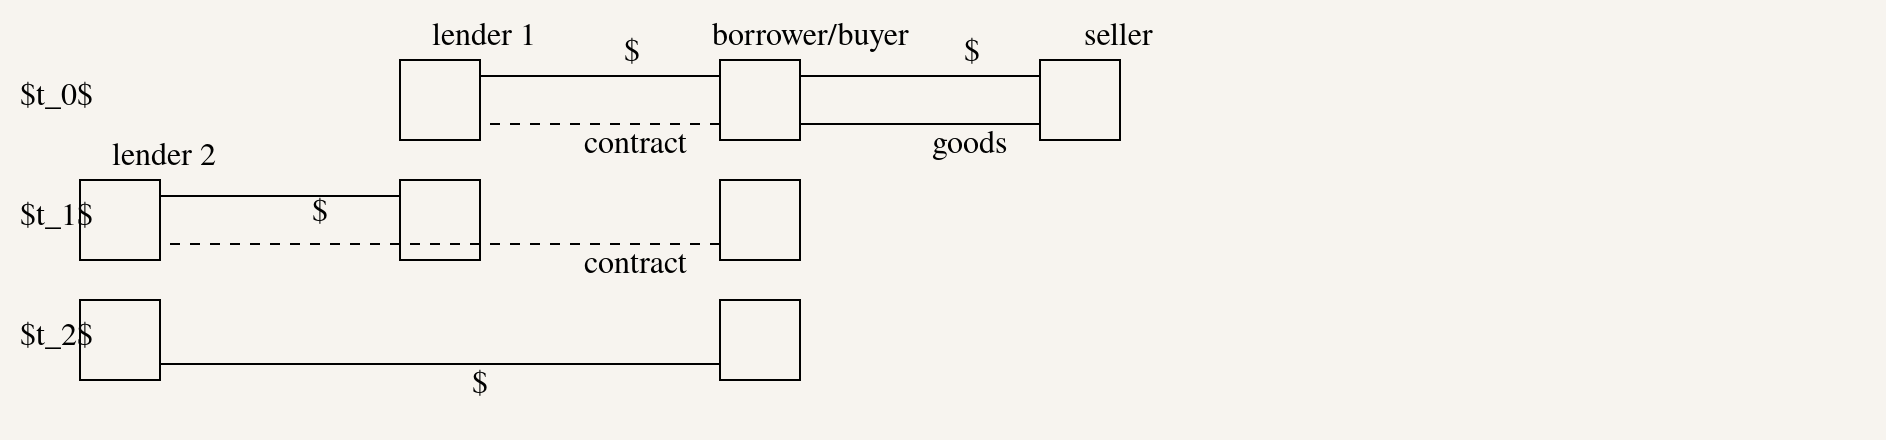
\includegraphics[scale=0.28]{01_introduction/png/contract_transactions}
% \caption{Contract Transactions}
% \label{fig:contract_transactions}
% \end{figure}
% 
% \begin{figure}[H]
% \centering
% \includegraphics[scale=0.28]{01_introduction/png/external_transactions}
% \caption{External Transactions}
% \label{fig:external_transactions}
% \end{figure}
% 
% \section{Error Correction}
% 
% \begin{figure}[H]
% \centering
% \includegraphics[scale=0.28]{01_introduction/png/exchange_only_feedback_schema}
% \caption{Exchange Only Feedback Model}
% \label{fig:exchange_only_feedback_schema}
% \end{figure}
% 
% Considering an economy where all other transaction categories have been eliminated, as
% indicated in figure 1.11, we can build a simple aggregate model as shown in figure 1.12.
% 
% \begin{figure}[H]
% \centering
% 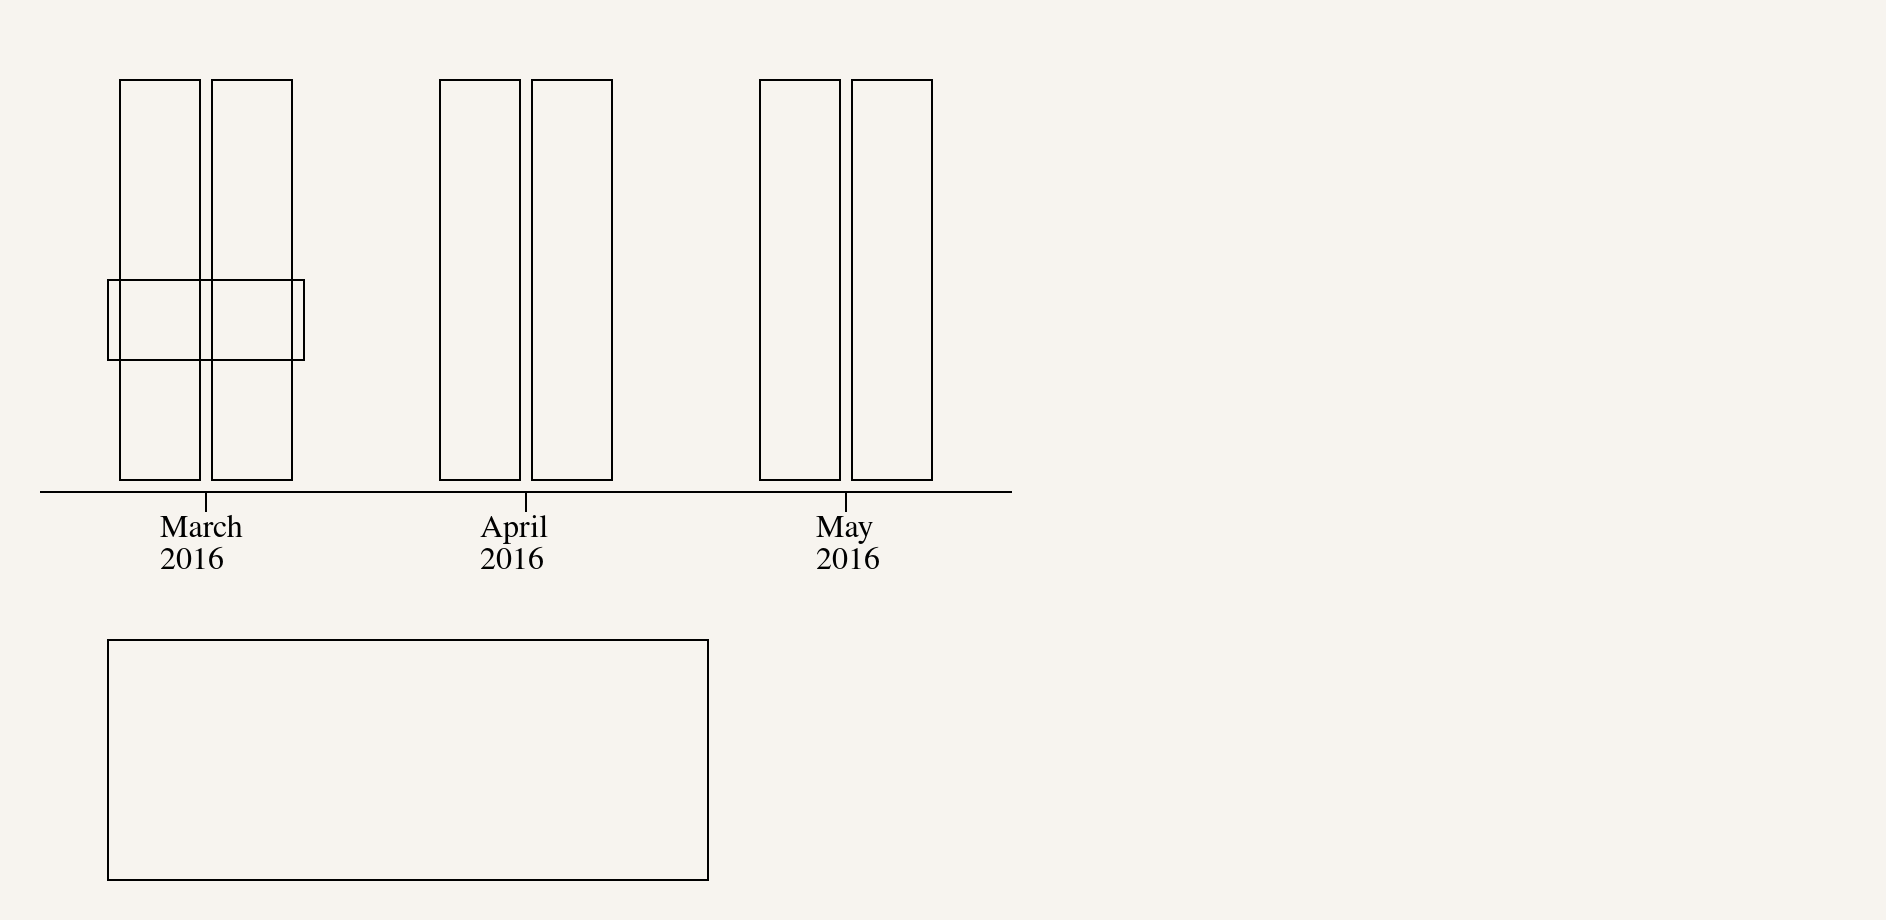
\includegraphics[scale=0.28]{01_introduction/png/exchange_only_aggregate_model}
% \caption{Exchange Only Aggregate Model}
% \label{fig:exchange_only_aggregate_model}
% \end{figure}
% 
% In periods 1 and 3, the unemployment rate, disregarding frictional unemployment, is zero.
% 
% So far the model is not constrained in any way. We apply to it an approximation of market behaviour,
% assuming that, in the absence of the monetary authority changing money supply and hence aggregate
% deman, that in each time period, the aggregate of prices \(p_i\) and quantities \(q_i\) adjust to
% market equilibrium, i.e. that there is not excess aggregate supply or excess aggregate demand. We
% now have a model which is the same as the 'simple model' we presented earlier.
% 
% \begin{figure}[H]
% \centering
% 
\includegraphics[scale=0.48]{01_introduction/png/blank}
% \caption{Equilibrium Aggregate Model}
% \label{fig:equilibrium_aggregate_model}
% \end{figure}
% 
% \begin{figure}[H]
% \centering
% 
\includegraphics[scale=0.28]{01_introduction/png/information_transmission}
% \caption{Information Transmission and Coding}
% \label{fig:information_transmission}
% \end{figure}
% 
% \begin{figure}[H]
% \centering
% 
\includegraphics[scale=0.48]{01_introduction/png/blank}
% \caption{Overbooking Model}
% \label{fig:overbooking}
% \end{figure}
% 
% \begin{figure}[H]
% \centering
% 
\includegraphics[scale=0.48]{blank}
% \caption{Aggregate Model with Overbooking}
% \label{fig:aggregate_overbooking}
% \end{figure}
% 
% \begin{figure}[H]
% \centering
% 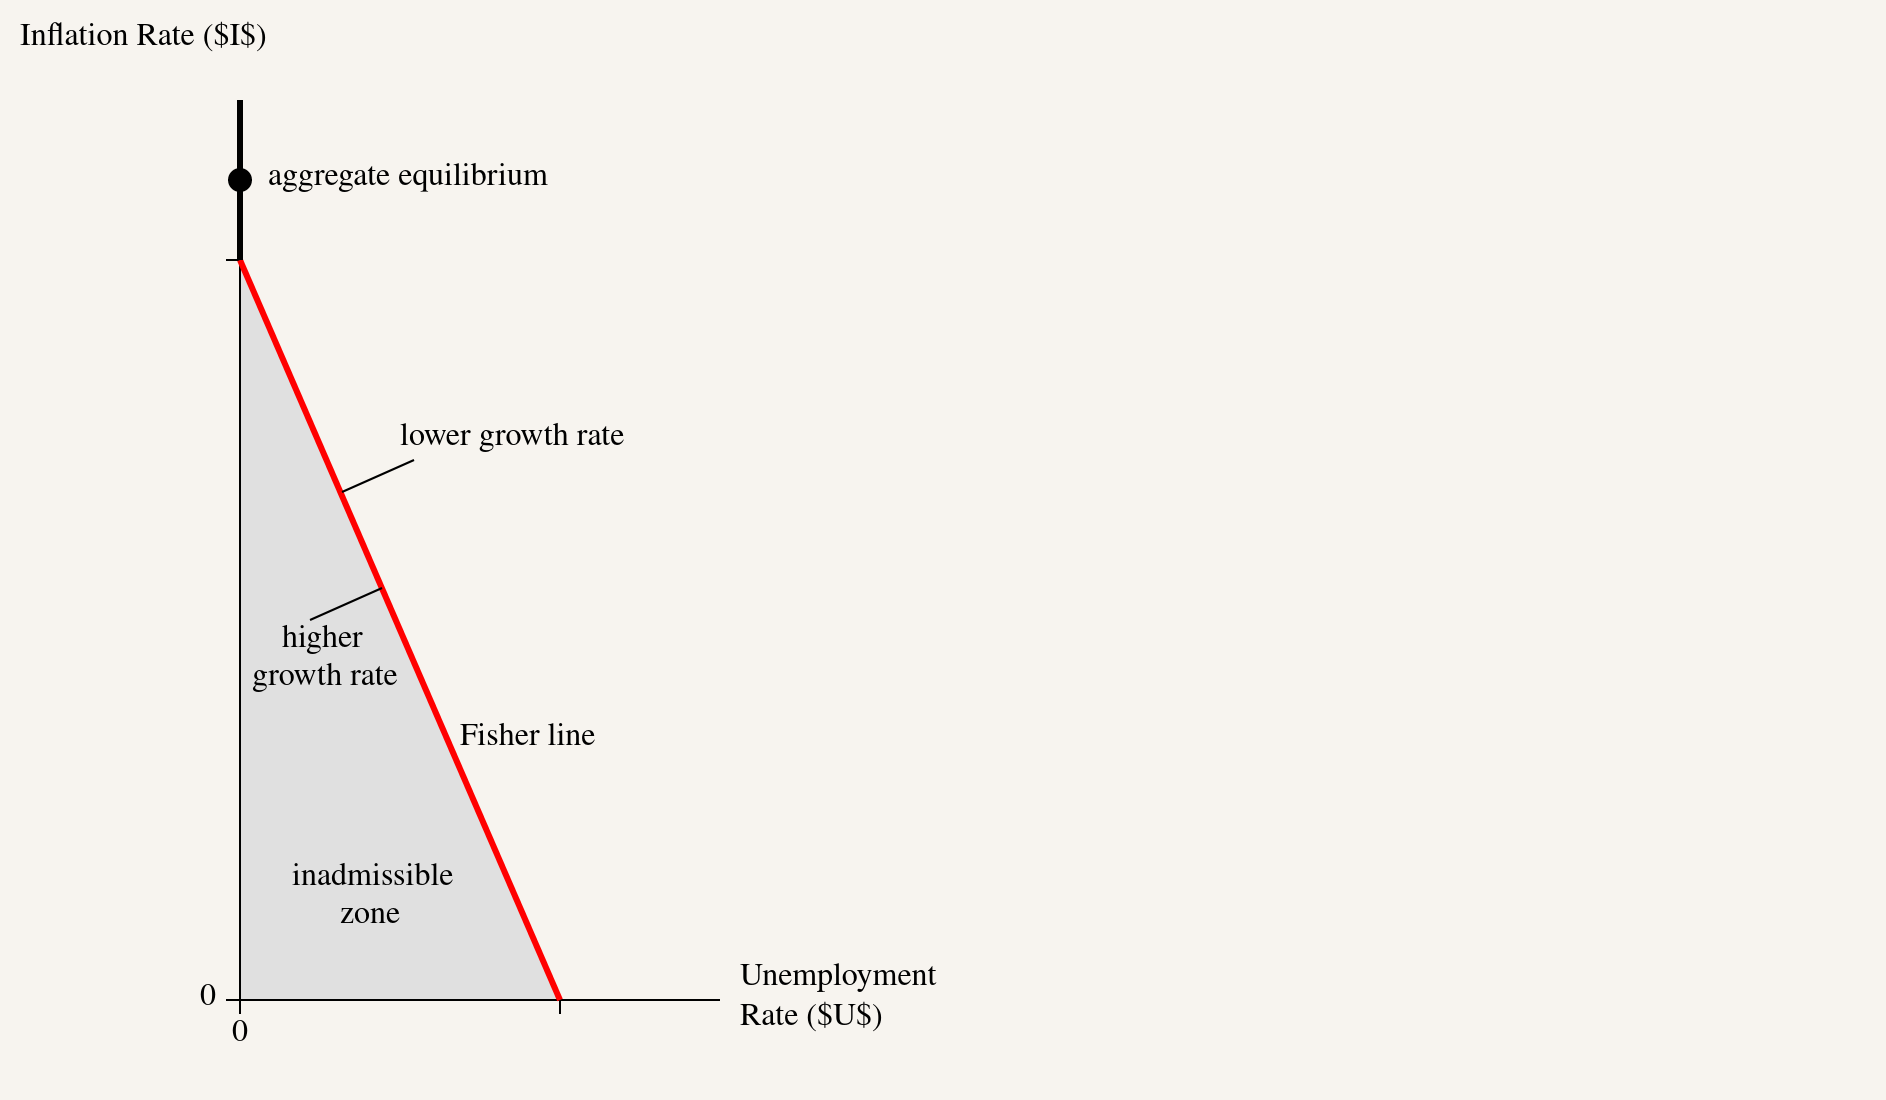
\includegraphics[scale=0.28]{/01/error_model}
% \caption{Error Model}
% \label{fig:error_model}
% \end{figure}
% 
% The most important implication is that markets only equilibriate in aggregate along the thick black
% line shown in Figure \ref{fig:error_model}, i.e. that market equilibriation an inflation rate
% greater than a certain positive value. Therefore our new problem is to design a currency which is
% controlled to maintain a state on the thick black line.
% 
% The critical control that a monetary authority has over a currency is
% 
% \begin{figure}[H]
% \centering
% 
\includegraphics[scale=0.48]{blank}
% \caption{Unemployment and Inflation for Selected Countries}
% \label{fig:ui_multi}
% \end{figure}
% 
% Figure \ref{fig:ui_multi} shows a relationship between unemployment and inflation data for selected
% countries that we expect to be linear when growth rates are relatively constant.
% 
% Therefore our new problem is to design a currency which is controlled to maintain a
% state on the thick black line. The critical control that a monetary authority has over a currency is
% through the supply of money and hence though aggregate demand and the inflation rate. In Figure
% \ref{fig:error_model} the left axis, inflation, is the control variable. The growth
% rate remains relatively exogenous.
% 
% To control aggregate demand we need to implement a feedback control loop with a set point above the
% he rate of inflation by a sufficient buffer (see Figure \ref{fig:error_model}) to handle variations
% in the system. This is best done by determining a value of from past data and then responding to
% changes in $F$, the
% total amount of money transacted during a period of time, which can easily be measured for a digital
% currency, backed up by unemployment surveys. The money supply can be precisely determined by
% indexing all payments by a index set by the monetary authority. This is done by making the payment
% value equal to the product of base account value and the index. In this way, the money in all
% accounts increases or decreases in exact proportion to all other accounts. This would appear to
% account users much the same as one sees interest payments affect the balance of bank accounts.
% 
% The error effect is caused by a faulty control system design, and explains why contemporary
% economies never achieve sustained market equilibriation or full employment. This result also
% 
% \subsection{Positive Feedback Instabilities}
% 
% \subsubsection{Time Transactions}
% 
% \subsection{Inflation Feedback}
% 
% Lending transactions cover all transactions lending contracts associated with an exchange
% transactions. Introducing lending transactions to our currency, we find a run-away positive feedback
% loop, where increases in inflation rates causes increases in real interest rates (Fisher effect),
% that if unconstrained result in the reduction of profits of productive enterprises that results in
% decreases in the growth rate and increases in the unemployment rate. This feedback can be identified
% in unemployment and inflation data. This feedback instability makes it impossible to sustainably
% maintain state on the black line. This feedback instability is caused by contracts nominated in
% nominal dollar values, and is solved by indexing contracts with a contract index along the lines of
% the Unidad de Formento in Chile. The result is that stable black line state can be maintained.
% 
% Introducing external transactions, we note that the exchange rate is exactly equal to the ratio of
% inflows of currency to outflows of currency. There exists a negative feedback process (Cassel) these
% inflows respond to deviations of the relative price levels in the two currencies to change the ratio
% of inflows to outflows to equilibriate the exchange rate to purchasing price parity. At PPP
% equilibrium, interactions between two currencies, become roughly equivalent to exchange
% transactions. This stable state, however, contradicts past records of exchange rates. We deal with
% this in the following paragraph.
% 
% \begin{figure}[H]
% \centering
% 
\includegraphics[scale=0.48]{blank}
% \caption{Inflation Feedback}
% \label{fig:inflation_feedback}
% \end{figure}
% 
% \subsection{Contract Transactions}
% 
% Contract transactions are used by banks to create bank accounts. Transfers of the value in bank
% accounts between different banks are accounted for by adjusting the debt relationship between those
% banks using contract transactions. Bank account debts are generally not completely backed by
% currency accounts. The result is a control problem, because if a large proportion money is held
% outside currency accounts, it because difficult for the currencies monetary authority to control
% aggregate demand.
% 
% Contractural transactions have both a stabilizing negative feedback effect through the exchange part
% of the transaction, but also can have destabilizing positive feedback runaway effects through
% increases in prices bring more participants into the market, thereby pushing up prices further.
% Whether the negative of positive feedback plays a dominant role depends on circumstances. Also,
% contract transactions are recursive and extensible and so it is possible that new kinds of
% transactions that can cause unpredictable interactions with the other classes of transactions, and
% therefore introduce unpredicted control problems. The danger becomes more acute if digital
% currencies that are designed specifically for Ponzi-like effects and interact with other currencies
% through an exchange rate are allowed to operate in the economy.
% 
% Financial bubbles occur when positive feedback becomes dominant, often resulting in sudden changes
% that are hard to predict and control. This is an example where the control problem is a result of
% the aggregate effects of markets (the plant) rather than the control system itself. These effects
% depend on the existance of contract transactions being implicitly, in the case of paper currency and
% other digital currencies, or explicitly.
% 
% \subsection{External Transactions}
% 
% \subsection{Interactions of Contract Transactions with External Transactions}
% 
% There is also considerable evidence that monetary flows across the external exchange rate boundary
% are volatile, and not subject to the stabilizing exchange rate feedback process present in exchange
% transactions. Contractural transactions have a sufficiently strong effect on the exchange rate such
% that it does not remain in equilibrium.
% 
% \subsection{Review of Transaction Interactions}
% 
% We now have the theoretical tools to build a digital currency that controls an economy for
% sustained and stable equilibriation of aggregate supply and demand. We require sufficiently large
% positive inflation rates to provide sufficient redundancy for the equilibriation of aggregate supply
% and demand. The results in the requirement to handle the interaction between exchange transactions
% and time transactions by requiring the use of a unit of account of constant purchasing power.
% 
% In the absence of capital flows, external currencies self-regulate. Contract transactions interact
% with exchange transactions by introducing the possibility of discontinuities which can disrupt the
% control of aggregate equilibrium. Contract transactions also interact with external transactions by
% destabilizing the self-regulation process of external transactions. Contract transactions also
% disrupt the control of aggregate demand.
% 
% \subsection{Control Solutions and Resiliance}
% 
% The two requirements for a stable equilibriating economy is the use of a unit of account for all
% contracts, and the prevention of capital transactions.
% 
% Calculating an accurate index for the unit of account requires a record of payments and goods
% categories for each exchange transaction. All repayments are associated with a contract frame, which
% determines at the time a contract is agreed upon, the money quantities to be repaid in units of
% account. Also, repayments can only be made to the account from which payments are originally made.
% 
% The exchange rate is set at purchasing price parity between the two currencies, which is the ratio
% of the price levels of the two currencies. The purchasing price parity should be close to the
% self-regulating exchange rate under the conditions specified above.
% 
% With no contract transactions, aggregate demand can be precisely and directly controlled through an
% exchange index.  The exchange index sets the purchasing value in accounts relative to an accounts
% base value. The purchasing value is a product of the base value and the exchange index. An increase
% in the exchange index increases the amount of all accounts in proportion. In general, the base value
% of an account is hidden, and account users will see increases in their account purchasing value
% closly in line with the inflation rate. The exchange index is the control variable and is generally
% calculated from the sum of payments for exchange transactions over a given period.  
% 
% \begin{figure}[H]
% \centering
% 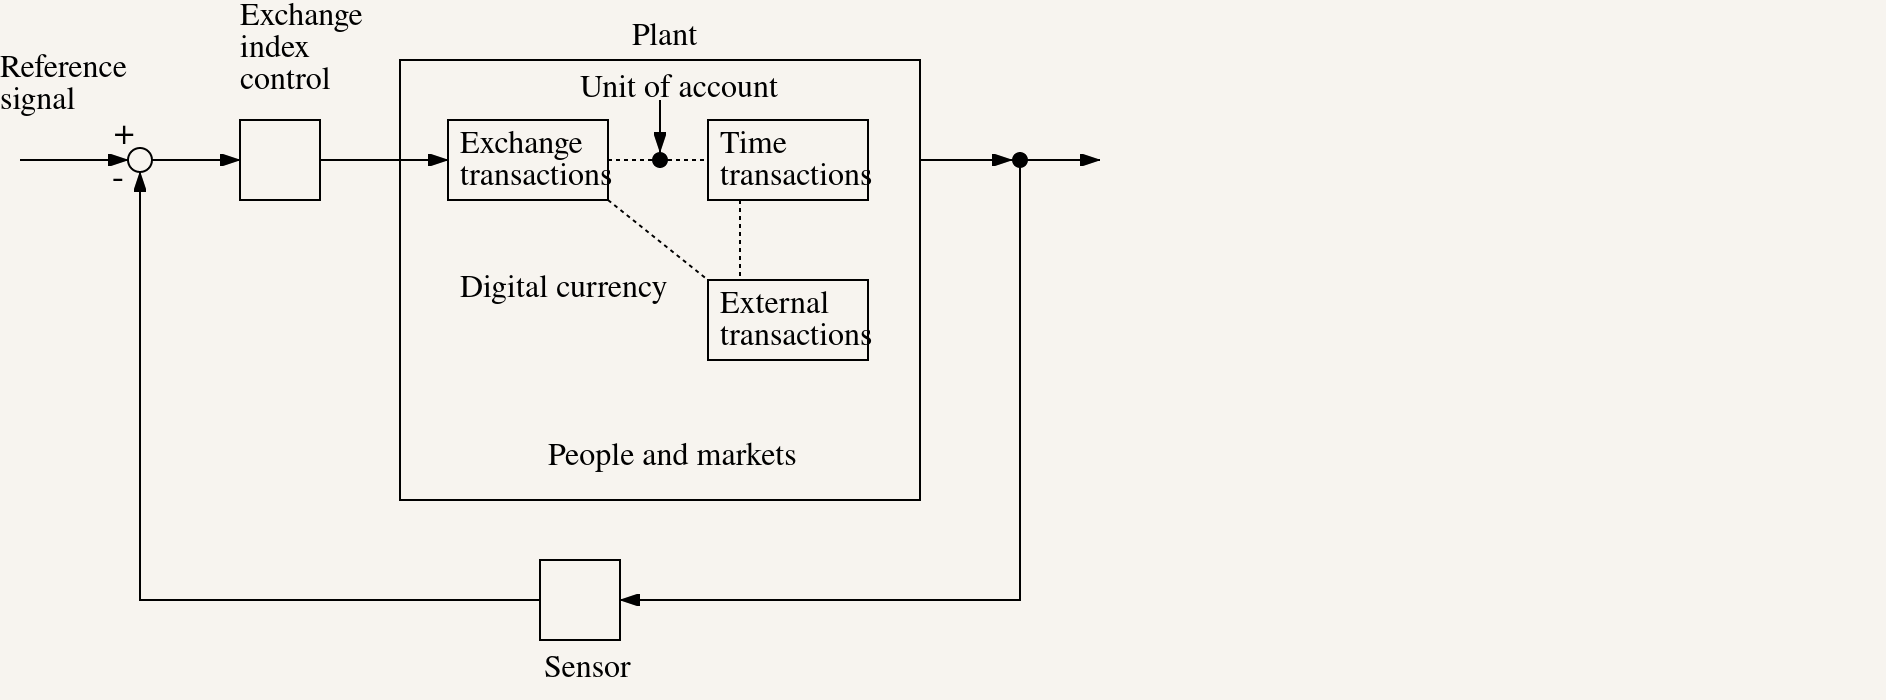
\includegraphics[scale=0.28]{/01/control_solution}
% \caption{Control System Design Solution}
% \label{fig:control_solution}
% \end{figure}
% 
% Figure \ref{fig:control_solution} shows the control solution, with the interactions between the
% classes of transactions designed to allow the aggregate price level to change without feedback
% interference, with contract transactions removed to prevent financial discontinuities and to allow
% the exchange rate to interact well with exchange and time transactions, and to allow direct control
% of aggregate demand through an exchange index.
